\documentclass{article}
\usepackage[utf8]{inputenc}
\usepackage[a4paper, margin=2.5cm]{geometry}
\usepackage{float}
\usepackage{graphicx}

\title{MLCourse-LU}
\author{YOUR STUDENT NUMBER HERE}
\date{Assignment 2}

\begin{document}

\maketitle



\begin{enumerate}
    \item % answer to question 1: Why does this model place "feathers" earlier in the tree than "airborne"?
    
    \item ...% answer to question 2: How could you find the instances in the dataset that end up in a particular leaf, but are misclassified?
    

    \item ... % answer to question 3: Why are the trees not always the same?
    
    \item ... % answer to question 4: Put a picture of a tree in your report that you think is particularly bad, and explain why it might have been fitted that way.
    
    
    \begin{figure}[H]
        \centering
        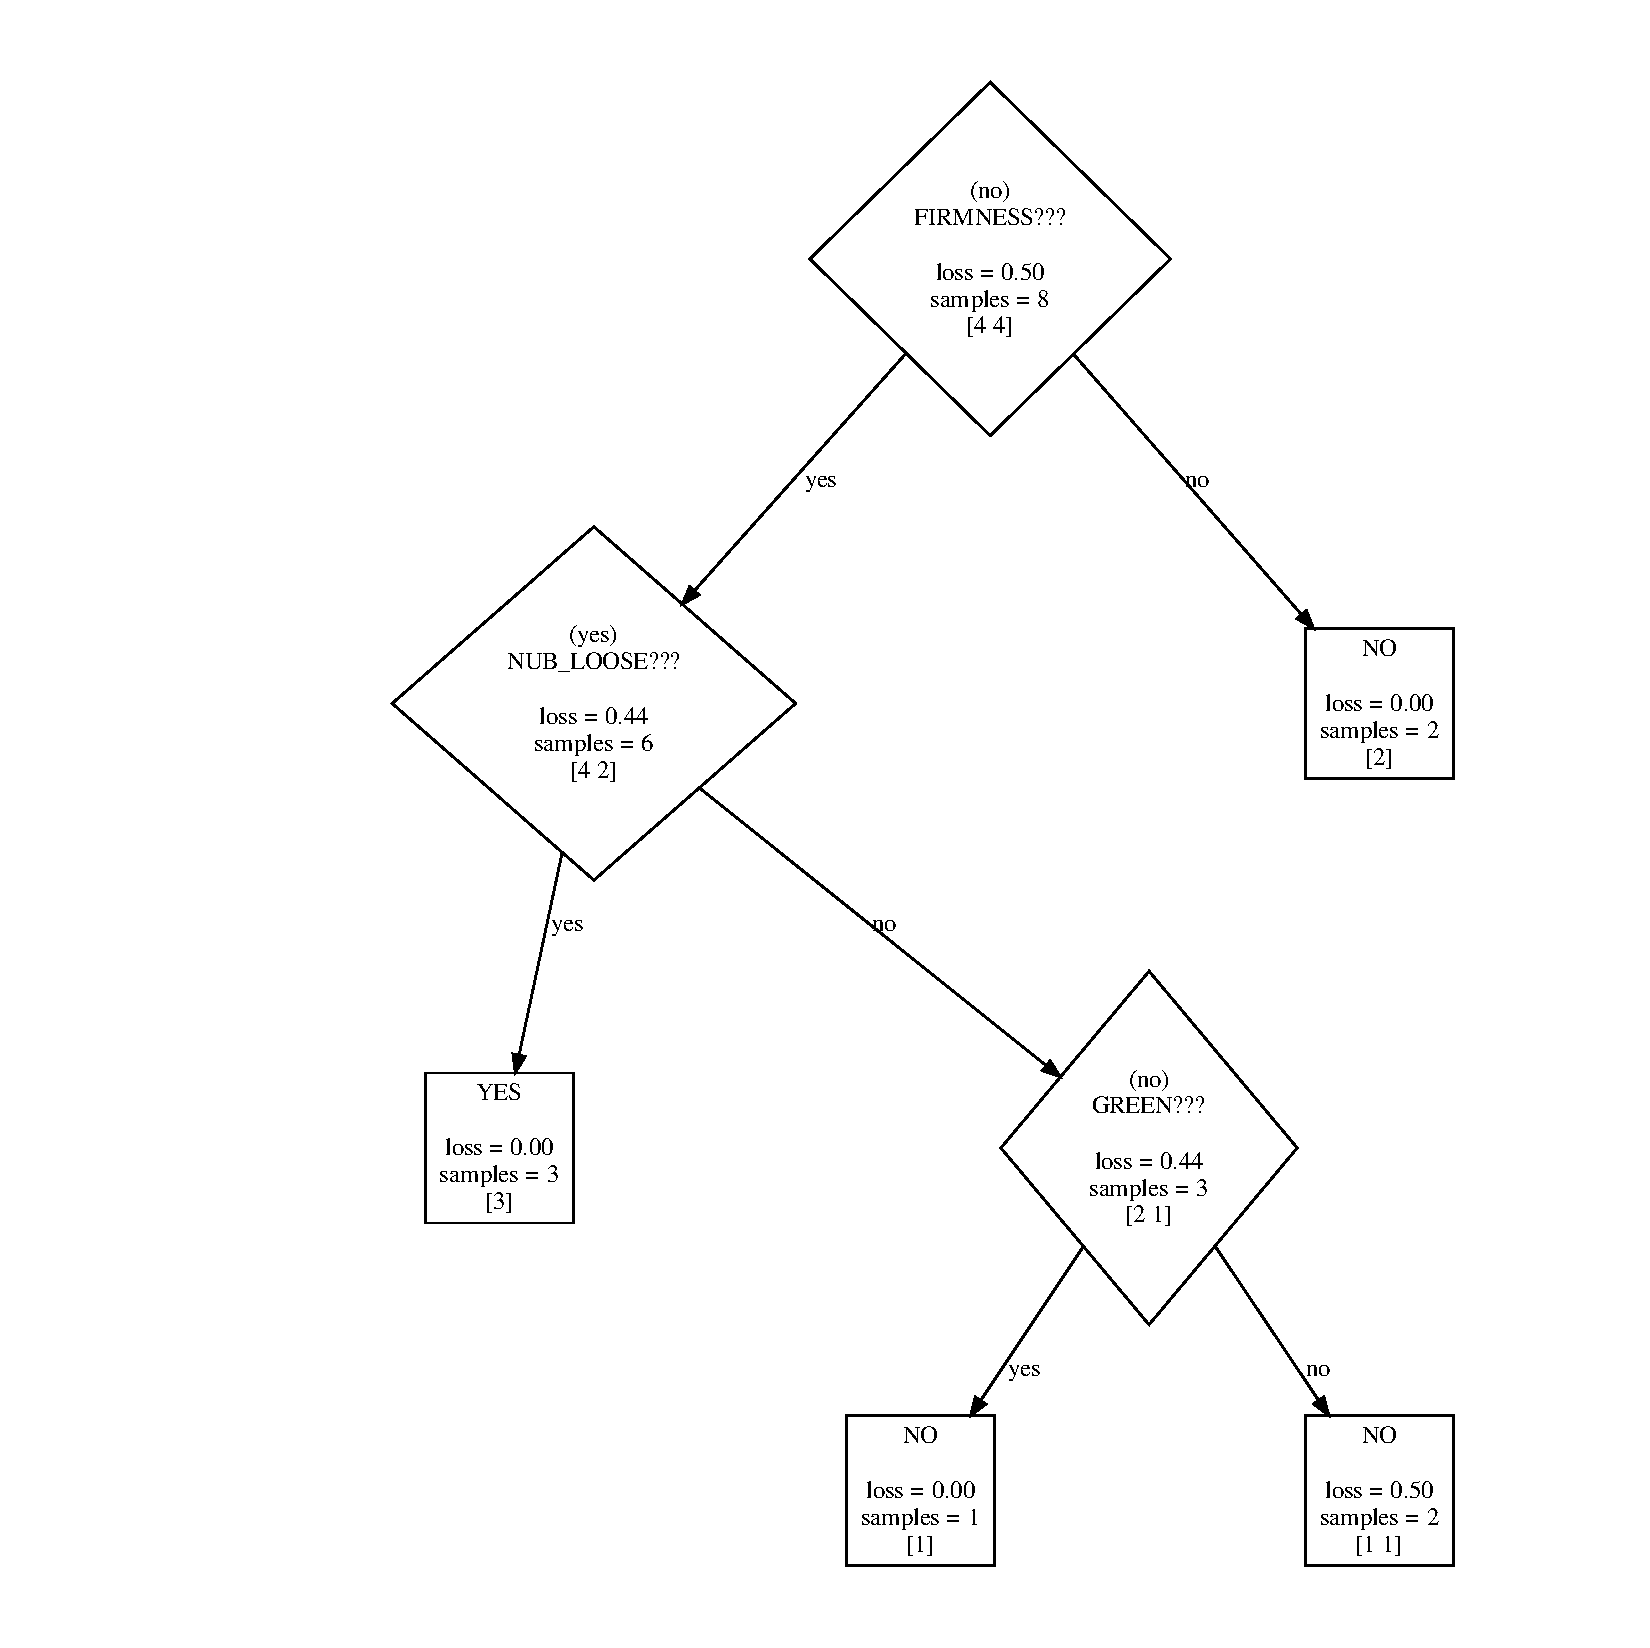
\includegraphics[width=\linewidth]{avocado.pdf}
        \caption{Explain what this figure represents}
        \label{fig:bad tree}
    \end{figure}


    
    \item ... % answer to question 5: Make a table comparing the different model/configurations. Report the mean and the standard deviation of the accuracy score.
    
    \begin{table}[H]
        \centering
        \begin{tabular}{l c c}
             \hline
             \textbf{Model + Loss} & \textbf{Mean} & \textbf{Standard Deviation} \\
             \hline
             ? & ? & ? \\
             ? & ? & ? \\
             ? & ? & ? \\
             ? & ? & ? \\
             ? & ? & ? \\
             \hline
        \end{tabular}
        \caption{Which of these/your setups works best?}
        \label{tab:model performance}
    \end{table}
    
    \item ... % answer to question 6: which would you prefer? A high-accuracy model with large standard deviation, or a somewhat lower accuracy model with lower standard deviation? Explain why.
    
    \item ... % answer to question 7: Experiment with different values of $k$. What is the effect on the accuracy and standard deviation of using larger or smaller $k$? Why do you think that is?
    
\end{enumerate}


\end{document}
